\documentclass[../main.tex]{subfiles}

\begin{document} %%%%%%%%%%%%%%%%%%%%%%%%%%%%%%%%%%%%%%%%%%%%%%%%%%%%%%%%%%%%
\section{Programación lineal} 
    La programción lineal (PL) es una herramienta para resolver problemas de optimización.

    \begin{example} Glapetto's Woodcarving (Juguetes de madera Giapetto)\\
        Giapetto's Woodcarving, Inc., manufactura dos tipos de juguetes de madera: soldados y trenes. Un soldado se vende en 27 dólares y requiere 10 dólares de materia prima. Cada soldado que se fabrica incrementa la mano de obra variable y los costos globales de Giapetto en 14 dólares. Un tren se vende en 21 dólares y utiliza 9 dólares de su valor en materia prima. Todos los trenes fabricados aumentan la mano de obra variable y los costos globales de Giapetto en 10 dólares. La fabricación de soldados y trenes de madera requiere dos tipos de mano de obra especializada: carpintería y acabados. Un soldado necesita dos horas de trabajo de acabado y una hora de carpinteria. Un tren requiere una hora de acabado y una hora de carpinteria. Todas las semanas, Giapetto consigue todo el material necesario, pero sólo 100 horas de trabajo de acabado y 80 de carpinteria. La demanda de trenes es ilimitada, pero se venden cuando mucho 40 soldados por semana. Giapetto desea maximizar las utilidades semanales (ingresos - costos). Diseñe un modelo matemático para la situación de Giapetto que se use para maximizar las utilidades semanales de la empresa.\\

        \textbf{Solución:}
        \begin{itemize}
            \item \textbf{Variables de decisión} 
                Se debe decidir cuántos soldados y trenes se deben fabricar cada semana. 
                \begin{equation}
                    \begin{split}
                        x_1 &= \text{ número de soldados fabricados por semana.}\\
                        x_2 &= \text{ número de trenes fabricados por semana.}
                    \end{split}
                \end{equation}
            \item \textbf{Función objetivo}
                Se desea maximizar las utilidades semanales de la empresa. 
                \begin{equation}
                    \begin{split}
                        \text{Ingresos por semana} &= \text{Ingresos por soldados} + \text{Ingresos por trenes} \\
                        &= \left(\frac{\text{dólares}}{\text{soldado}}\right) \cdot \left(\frac{\text{soldados}}{\text{semana}}\right) + \left(\frac{\text{dólares}}{\text{tren}}\right) \cdot \left(\frac{\text{trenes}}{\text{semana}}\right)  \\
                        &= 27 \cdot x_1 + 21 \cdot x_2
                    \end{split}
                \end{equation}

                Asimismo
                \begin{equation}
                    \begin{split}
                        \text{Costo de la materia prima a la semana} &= 10 \cdot x_1 + 9 \cdot x_2 \\
                        \text{Otros costos variables a la semana} &= 14 \cdot x_1 + 10 \cdot x_2
                    \end{split}
                \end{equation}

                Entonce, se quiere maximizar
                \begin{equation}
                    \begin{split}
                        \text{Utilidades semanales} &= \text{Ingresos semanales} - \text{Costos semanales} \\
                        &= 27 \cdot x_1 + 21 \cdot x_2 - (10 \cdot x_1 + 9 \cdot x_2 + 14 \cdot x_1 + 10 \cdot x_2) \\
                        &= 3 \cdot x_1 + 2 \cdot x_2
                    \end{split}
                \end{equation}

                La función objetivo es
                \begin{equation}
                        \text{Maximizar } z =  3 \cdot x_1 + 2 \cdot x_2
                \end{equation}

            \item \textbf{\underline{Restricciones:}}
                \begin{itemize}
                    \item Restricción 1: Se puede usar cada semana no más de 100 horas de tiempo de acabado.
                    \item Restricción 2: Cada semana se puede usar no más de 80 horas de tiempo de carpintería.
                    \item Restricción 3: Debido a la demanda limitada, cuando mucho se debe producir cada semana 40 soldados.
                \end{itemize}

                La cantidad de materia prima en existencia es ilimitada, asi que no hay restricción alguna relacionada con eso.

                Para expresar la restricción 1 de acuerdo con $x_1$ y $x_2$.
                \begin{equation}
                    \begin{split}
                        \frac{\text{Total de horas de acabado}}{\text{Semana}} &= \left(\frac{\text{horas de acabado}}{\text{soldado}}\right) \cdot \left(\frac{\text{soldados frabricados}}{\text{semana}}\right) \\ & + \left(\frac{\text{horas de acabado}}{\text{tren}}\right) \cdot \left(\frac{\text{trenes frabricados}}{\text{semana}}\right)  \\
                        &= 2 \cdot x_1 + 1 \cdot x_2 \\
                    \end{split}
                \end{equation}

                Entonces, la restricción 1 se puede expresar como
                \begin{equation}
                    2 \cdot x_1 + 1 \cdot x_2 \leq 100
                \end{equation}

                Para la restricción 2 en términos de $x_1$ y $x_2$.
                \begin{equation}
                    \begin{split}
                        \frac{\text{Total de horas de carpintería}}{\text{Semana}} &= \left(\frac{\text{horas de carpintería}}{\text{soldado}}\right) \cdot \left(\frac{\text{soldados fabricados}}{\text{semana}}\right) \\ & + \left(\frac{\text{horas de carpintería}}{\text{tren}}\right) \cdot \left(\frac{\text{trenes fabricados}}{\text{semana}}\right)  \\
                        &= 1 \cdot x_1 + 1 \cdot x_2 \\
                    \end{split}
                \end{equation}

                Entonces, la restricción 2 se puede expresar como
                \begin{equation}
                    1 \cdot x_1 + 1 \cdot x_2 \leq 80
                \end{equation}

                Para la restricción 3 en términos de $x_1$ y $x_2$.
                \begin{equation}
                    x_1 \leq 40
                \end{equation}

            \item \textbf{Restricciones de signo}
                \begin{equation}
                    \begin{split}
                        x_1 &\geq 0 \\
                        x_2 &\geq 0
                    \end{split}
                \end{equation}
            \label{item:ejemplo_giapetto}
        \end{itemize}

        Presentamos el modelo de PL para el problema de Giapetto's Woodcarving.
        \begin{equation}
            \text{Maximizar } z =  3 \cdot x_1 + 2 \cdot x_2
        \end{equation}

        sujeto a
        \begin{equation}
            \begin{aligned}
            2x_1 + x_2 &\leq 100 && \text{(Restricción de acabado)}\\
            x_1 + x_2 &\leq 80 && \text{(Restricción de carpintería)}\\
            x_1 &\leq 40 && \text{(Restricción de demanda)}\\
            x_1 &\geq 0 && \text{(Restricción de signo)}\\
            x_2 &\geq 0 && \text{(Restricción de signo)}
            \end{aligned}
        \end{equation}

        Ahora vamos a resolver el problema de Giapetto's Woodcarving.

        \begin{figure}[ht]
            \centering
                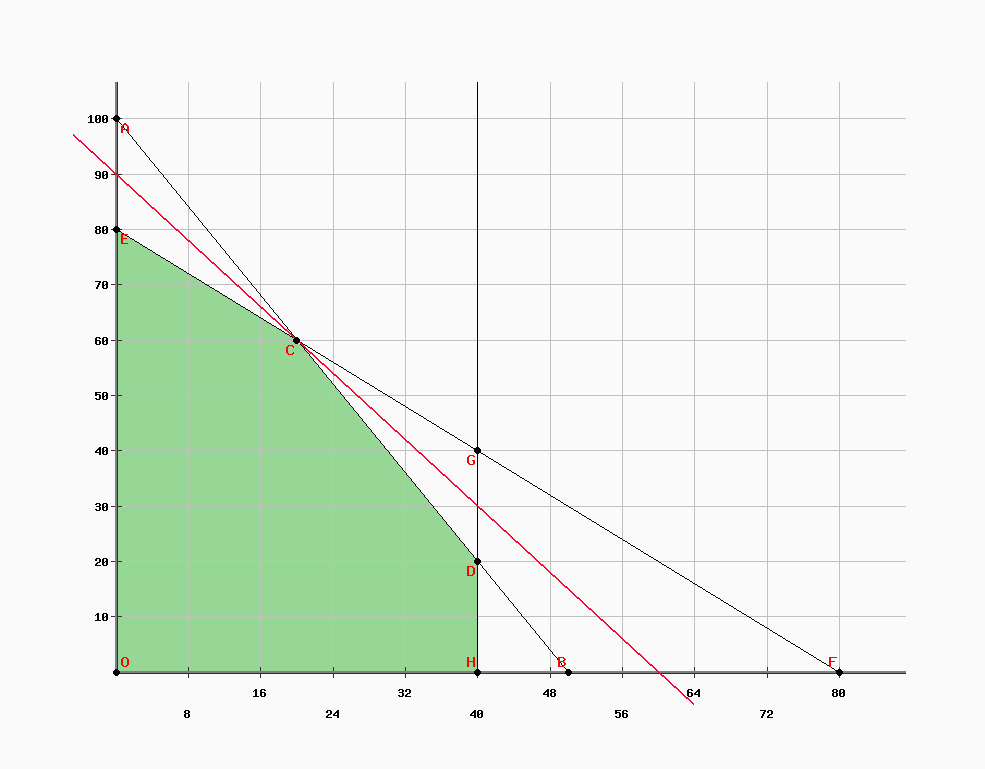
\includegraphics[width=1\textwidth]{./images/pl_grafico.png}
                \caption{Región factible para el problema de Giapetto's Woodcarving.}
            \label{fig:figura1}
        \end{figure}

        Usando la región factible se busca la solución óptima, la cual es el punto de la región factible con el valor más grande de $z = 3 \cdot x_1 + 2 \cdot x_2$. En este caso, la solución óptima es, recta roja gráfico, punto C:
        \begin{equation}
            x_1 = 20, \quad x_2 = 60, \quad z = 180
        \end{equation}

                  
    \end{example}

    \begin{teorema}{Problema de programación lineal}{}
        Un problema de programación lineal (PL) es un problema de optimización para el cual se efectúa lo siguiente:
        \begin{enumerate}
            \item Se intenta maximizar (minimizar) una función lineal de las variables de decisión. La función lineal se llama \textbf{función objetivo}.
            \item Los valores de las variables de decisión deben satisfacer un conjunto de restricciones. Cada restricción debe ser una ecuación lineal o una inecuación lineal.
            \item Se relaciona un \textit{restricción de signo} con cada variable de decisión.
        \end{enumerate}
    \end{teorema}
    
    \subsection{Regiones factibles y solución óptima}
        \begin{definition} \textbf{(Región factible)}
            La región factible para una PL, es el conjunto de todos los puntos que satisfacen las limitaciones y las restricciones de signo de la PL.
        \end{definition}

        \begin{definition} \textbf{(Solución óptima)}
            Para un problema de maximización, una solución óptima para una PL es un punto con el valor de la función objetivo más grande en la región factible. De igual manera, para un problema de minimización, una solución óptima es un punto con el valor de la función objetivo más pequeño en la región factible.
        \end{definition}

    \subsection{Restricciones activas}
        \begin{definition} \textbf{(Restricciones activas)}
            Una restricción es activa u obligatoria si tanto el primero como el segundo miembro de las restricciones son iguales cuando los valores óptimos de las variables de decisión se sustituyen en la restricción.
        \end{definition}

        \begin{definition} \textbf{(Restricciones inactiva)}
            Una restricción es inactiva si no son iguales el primero y el segundo miembro de la restricción cuando los valores óptimos de las variables de decisión se sustituyen en la restricción.
        \end{definition}

        En el Ejemplo \ref{item:ejemplo_giapetto}, 
        \begin{equation}
            \begin{aligned}
            2 \cdot \overset{\underbrace{x_1}}{(20)} + \overset{\underbrace{x_2}}{(60)} &= 100  && \text{(Restricción activa)}\\
            (20) + (60) &= 80 && \text{(Restricción activa)}\\
            (20) &\leq 40 && \text{(Restricción inactiva)}
            \end{aligned}
        \end{equation}

    \subsection{Casos especiales}
        Tres tipos de PL que no tienen solución óptima única:
        \begin{enumerate}
            \item Tienen un número infinito de soluciones óptimas. (\textit{soluciones óptimas múltiples o alternativas})
            \item No tienen soluciones factibles. (\textit{soluciones no factibles})
            \item Son no acotadas: hay puntos en la región factible con valores $z$ arbitrariamente grandes (en problemas de maximización).
        \end{enumerate}

        \begin{example}
            
        \end{example}
\end{document}  %%%%%%%%%%%%%%%%%%%%%%%%%%%%%%%%%%%%%%%%%%%%%%%%%%%%%%%%%%%%%
